\documentclass[oneside,10pt]{swissi}

\addbibresource{4-bib/2-bib.bib}
\newcommand{\papertitle}{Generic AI-DLT Enterprise System}
\newcommand{\papersubtitle}{Architecture and methodology for scalable domain adaptation from a unified core framework}

\newcommand{\papercitationauthors}{Kurz, W. and Malara, M. and Dedi{\'c}, V.}

\newcommand{\paperauthors}{%
  Walter Kurz\textsuperscript{1}%
  , Michel Malara\textsuperscript{1}%
  , Velimir Dedi{\'c}\textsuperscript{1}%
}

\newcommand{\paperaffiliations}{%
  \textsuperscript{1}Swissi Institute for AI,
  \href{mailto:kurz@swissi-ai.institute}{kurz@swissi-ai.institute};
  \href{mailto:malara@swissi-ai.institute}{malara@swissi-ai.institute};
  \href{mailto:dedic@swissi-ai.institute}{dedic@swissi-ai.institute}%
}

\newcommand{\paperdeclarationaffiliations}{%
  \begin{tabular}[t]{@{}l@{}}
    \textsuperscript{1}Swissi Institute for AI,
    \href{mailto:kurz@swissi-ai.institute}{kurz@swissi-ai.institute};
    \href{mailto:malara@swissi-ai.institute}{malara@swissi-ai.institute};
    \href{mailto:dedic@swissi-ai.institute}{dedic@swissi-ai.institute}%
  \end{tabular}%
}

\newcommand{\papercorresponding}{%
  Walter Kurz,
  \href{mailto:kurz@swissi-ai.institute}{kurz@swissi-ai.institute},
  \href{https://orcid.org/0009-0006-8045-4775}{ORCID 0009-0006-8045-4775}%
}

\newcommand{\paperfunding}{%
  This research received no external funding.%
}
\newcommand{\paperconflictsofinterest}{%
  The authors declare no conflicts of interest.%
}
\newcommand{\paperdataavailability}{%
  The data and code supporting this article are available from the corresponding author on reasonable request.%
}
\newcommand{\paperaitools}{%
  Generative AI tools were used for editorial work only, such as language editing and formatting, in accordance with international scientific standards. The authors verified the content and remain fully responsible for the article.%
}
\newcommand{\paperauthorcontributions}{%
  All authors contributed equally to this article.%
}

\providecommand{\swIncludeAuthorExamples}{}

\title{\papertitle \\[0.35em]
\normalsize \papersubtitle}

\author{{\fontsize{8}{10}\selectfont\paperauthors}\\[0.9em]
{\scriptsize\paperaffiliations}}
\date{\vspace{1.5em}}

\begin{document}
\maketitle

\begin{abstract}
The objective of this study is to define a compliance-first, conceptually generalisable architecture for a multi-agent artificial intelligence platform integrated with distributed ledger technology, designed to be domain-, deployment-, and vendor-agnostic. It addresses a persistent shortcoming in current AI deployments, where compliance is often treated as a secondary concern, applied retroactively through prompt engineering rather than embedded within the foundational design. The proposed model encodes regulatory, governance, and ESG requirements into an objective-under-constraints framework, ensuring that all specialised agents operate within legally admissible and verifiably auditable parameters prior to any domain-specific implementation. A DAG-based verification layer is incorporated to enable scalable, low-latency, and cost-efficient operation while preserving evidentiary integrity. The analysis evaluates the feasibility of this conceptual model to support sustainable, rapid-deployment vertical applications without inducing vendor lock-in, preserving operational neutrality, and ensuring environmental accountability. The findings suggest that integrating compliance, ESG metrics, and agent specialisation at the architectural level provides a transferable foundation for cross-domain AI–DLT infrastructures.
\end{abstract}

\keywords{Compliance-first AI, Multi-agent systems, Distributed ledger technology, Directed acyclic graph, Regulation by design, ESG integration, Domain-agnostic architecture, Deployment-agnostic architecture, Vendor-agnostic architecture, Objective-under-constraints}

\bigskip

\section{Introduction}\label{sec1}

Contemporary consumer-facing artificial intelligence deployments are dominated by large language models (LLMs) and related generative architectures, typically accessed through proprietary API endpoints.\cite{aiindex2025economy,openai_api_models} In such systems, the generated output itself constitutes the primary product.\cite{aiindex2025economy}

Internal optimisation targets coherence, syntactic precision, and surface-level factuality, achieved through prompt engineering, instruction tuning, retrieval-augmented generation (RAG) pipelines, and post-processing moderation.\cite{schulhoff2024prompt,longpre2023flan,ouyang2022instruct,lewis2020rag,openai_moderation_docs} These mechanisms are effective in improving immediate relevance and reliability, particularly where the value of the system is measured by the quality of a single response.\cite{lewis2020rag,ouyang2022instruct}

Such output-centric architectures exhibit structural limitations in enterprise-scale, multi-agent systems operating in regulated domains.\cite{nist_ai_rmf_2023}

In consumer deployments, compliance, ethical alignment, and environmental, social, and governance (ESG) considerations are typically applied as non-binding guidelines or post hoc filters rather than embedded constraints.\cite{nist_ai_rmf_2023}

Provider control is exercised primarily through model training choices and prompt manipulation, which provides no systemic assurance that outputs, or the intermediate reasoning steps producing them, comply with procedural, legal, or evidentiary requirements.\cite{eu_ai_act_2024,nist_ai_rmf_2023}

From the provider’s perspective, this optimisation objective can be formalised as the constrained problem in Equation~\eqref{eq:consumer-llm-obj}, where the aim is to maximise perceived output quality within bounded constraints on compliance, factual accuracy, user-perceived helpfulness, stylistic acceptability, safety, and latency.
\begin{align}
\max_{y \in \mathcal{Y}} \quad & Q_{\text{user}}(y, x, \theta) \label{eq:consumer-llm-obj} \\
\text{s.t.} \quad
& C_{\text{policy}}(y) = 1 & \text{(compliance with policies and applicable laws)} \nonumber \\
& C_{\text{factual}}(y, \mathcal{K}) \geq \tau_f & \text{(factual correctness relative to knowledge base $\mathcal{K}$)} \nonumber \\
& C_{\text{context}}(y, x) \geq \tau_c & \text{(alignment with inferred user intent)} \nonumber \\
& C_{\text{style}}(y) \geq \tau_s & \text{(stylistic acceptability and engagement quality)} \nonumber \\
& C_{\text{safety}}(y) \geq \tau_{\sigma} & \text{(safety and risk minimisation)} \nonumber \\
& T(y) \leq \tau_t & \text{(latency limit for output delivery)} \nonumber
\end{align}

Here, $y \in \mathcal{Y}$ denotes the output text sequence generated by the model in response to the input prompt $x$, with $\theta$ representing the model parameters. The scalar utility function $Q_{\text{user}}$ estimates the perceived output quality from the end-user’s perspective. The constraint $C_{\text{policy}}$ enforces compliance with provider policies and applicable legal frameworks. Factual correctness is measured by $C_{\text{factual}}$ relative to a knowledge base $\mathcal{K}$, bounded below by a threshold $\tau_f$. Contextual alignment with inferred user intent is expressed as $C_{\text{context}}$ with threshold $\tau_c$, while $C_{\text{style}}$ ensures stylistic and rhetorical acceptability above threshold $\tau_s$. Safety and reputational risk minimisation are modelled through $C_{\text{safety}}$ with threshold $\tau_{\sigma}$, and $T(y)$ denotes the total generation latency, constrained by $\tau_t$.

Enterprise-grade AI, by contrast, functions as a delegated agent on behalf of an organisation, whether corporate, governmental, medical, or otherwise, and must operate within a normative framework.\cite{handbook_normative_mas,wooldridge2009} In such contexts, accuracy of output is necessary but insufficient for admissibility.\cite{eu_ai_act_2024} All actions and decisions must be bounded by a formally defined \emph{objective-under-constraints} environment in which compliance, ESG adherence, and procedural validity are structural guarantees rather than aspirational properties.\cite{nist_ai_rmf_2023,eu_ai_act_2024} This mirrors the legal and contractual obligations of human actors, whose conduct is constrained by performance requirements as well as enforceable compliance obligations.\cite{nist_ai_rmf_2023}

Within this frame, generative models, including LLMs, are best understood as modular components within a larger multi-agent architecture, rather than as the defining element of the system.\cite{wooldridge2009} The proposed approach comprises two co-dependent layers: a modular, role-specific multi-agent system capable of both persistent and ad hoc committee formation for continuous and event-driven tasks; and a distributed ledger infrastructure, incorporating a directed acyclic graph (DAG) verification layer to deliver low-latency, tamper-evident auditability.\cite{handbook_normative_mas,nistir8202,baird2016hashgraph} This design is deliberately deployment- and vendor-agnostic, enabling heterogeneous AI modules, generative or otherwise, to be integrated without compromising compliance or scalability.\cite{nist_ai_rmf_2023,nistir8202}

\section{Related Work and Research Gap}\label{sec2}
\subsection{Multi-Agent Architectures in AI Systems}

Multi-agent systems (MAS) have a long history in distributed problem solving, coordination, and planning, with established mechanisms for task allocation and cooperation such as the Contract Net Protocol and cooperative planning pipelines.\cite{smith1980contractnet,torreno2017survey} Classical accounts describe autonomous, locally rational agents that coordinate through negotiation, commitments, or shared plans to achieve global objectives in heterogeneous environments.\cite{jennings1998roadmap,wooldridge2009} This tradition forms the basis of many contemporary frameworks, which adopt the decomposition of complex objectives into role-specific competencies, local decision making, and explicit protocols for inter-agent communication.\cite{jennings1998roadmap,torreno2017survey}

Recent advances in large language models (LLMs) have prompted renewed interest in agentic architectures that use LLMs as planning, communication, and tool-use primitives. These support conversational teams and orchestration layers, as shown by frameworks such as AutoGen, which enable conversation-programmed teams of specialised agents, and by role-playing and workflow-based approaches (e.g., CAMEL, MetaGPT), which demonstrate how division of labour and inter-agent critique can improve performance on open-ended tasks.\cite{wu2023autogen,li2023camel,hong2023metagpt} Methodologically related patterns like ReAct integrate chain-of-thought reasoning with action selection, reinforcing tool-using agent designs.\cite{yao2023react}

Beyond research prototypes, developer toolchains provide agent modules for domain-specific pipelines. For example, LangChain-based agents have been applied in data- and tool-integrating systems such as bilingual real-estate advisory assistants, illustrating the accessibility, but also the variability, of engineering practices in current agent stacks.\cite{haurum2024langchain}

Most of these systems are assessed primarily on functional metrics such as task success, sample efficiency, or benchmark scores, with embedded compliance properties rarely enforced at the orchestration layer. This gap is reflected in the creation of dedicated safety and trustworthiness benchmarks for LLM agents, which document frequent policy violations and limited risk-awareness even when task outcomes meet performance targets.\cite{yuan2024rjudge,levy2024stwebagentbench} Surveys of LLM-based MAS and of LLM security and privacy similarly characterise the field as performance-driven, with governance and assurance positioned as peripheral rather than architectural concerns.\cite{li2024llmmas_survey,yao2024llmsecpriv} These findings motivate the design of architectures in which compliance, procedural validity, and auditability are encoded as binding constraints on inter-agent coordination, rather than implemented through external monitoring after deployment.

\subsection{Compliance-by-Design in AI}

Compliance-by-design, also referred to as regulation-by-design, is embedded in European data protection law through the principle of \emph{data protection by design and by default} (DPbDD), which requires ex ante technical and organisational measures by controllers (Article~25 GDPR) and is elaborated in the European Data Protection Board’s Guidelines~4/2019.\cite{gdpr2016,edpb2020art25} Contemporary AI governance frameworks extend this preventive approach: the EU Artificial Intelligence Act adopts a risk-based regime in which classification and obligations depend on risk level (notably Article~6 and Annex~III for high-risk applications), while the NIST AI Risk Management Framework (AI~RMF~1.0) structures governance, mapping, measurement, and management functions across the AI lifecycle.\cite{eu_ai_act_2024,nist_ai_rmf_2023}

For high-risk AI systems, the AI Act sets both design-time and run-time requirements that operationalise compliance-by-design. These include a documented, lifecycle \emph{risk management system} (Article~9); \emph{data and data governance} controls for training, validation, and testing datasets (Article~10); \emph{technical documentation} demonstrating conformity (Article~11); \emph{logging} capabilities for traceability and supervision (Article~12); \emph{transparency} obligations toward deployers (Article~13); \emph{human oversight} mechanisms (Article~14); and thresholds for \emph{accuracy, robustness, and cybersecurity} (Article~15).\cite{eu_ai_act_2024} Conformity is reinforced through \emph{conformity assessment} procedures (Article~43), post-market \emph{monitoring and incident reporting} (Articles~72–73), and registration in an EU database for traceability (Articles~49,~71). Together, these measures embed auditability into orchestration rather than treating it as an external control.\cite{eu_ai_act_2024} Complementary standards such as ISO/IEC~42001:2023 (AI management systems) and ISO/IEC~23894:2023 (AI risk management guidance) codify organisational processes that support such embedding at scale.\cite{iso42001,iso23894}

In practice many implementations remain model-centric: compliance mechanisms are attached to single-model pipelines via pre-deployment documentation and post hoc audits, rather than enforced as binding constraints across system orchestration.\cite{raji2020accountability,costanzachock2022whoaudits} Reporting artefacts such as \emph{model cards} and \emph{datasheets for datasets} improve transparency but do not, on their own, guarantee procedural validity under operational conditions or cross-component accountability in complex deployments.\cite{mitchell2019modelcards,gebru2021datasheets} Distributed, multi-agent ecosystems amplify these gaps because compliance must propagate consistently across inter-agent communication, task delegation, and decision rights. Current surveys and risk frameworks describe assurance in such contexts as an unresolved socio-technical challenge, reinforcing the need to integrate governance and oversight into orchestration logic rather than relying solely on downstream monitoring.\cite{yao2024llmsecpriv,nist_ai_rmf_2023}

\subsection{Distributed Ledger Technology for Verification}

Distributed ledger technology (DLT) is widely used to secure data integrity, provenance, and auditability by maintaining append-only, tamper-evident records in adversarial settings.\cite{nistir8202,nakamoto2008} These guarantees are realised through hash-chaining and authenticated data structures, such as Merkle trees, which enable efficient inclusion and append-only proofs, as demonstrated in transparency-log systems for public auditing.\cite{rfc9162,crosby2009,tomescu2019} Enterprise-grade, permissioned platforms such as Hyperledger Fabric extend these primitives with identity management, endorsement policies, and configurable consensus, providing fine-grained access control and verifiable transaction histories.\cite{androulaki2018}

Conventional blockchains impose a linear order of blocks, simplifying verification but constraining throughput and latency.\cite{nistir8202,nakamoto2008} Directed acyclic graph (DAG) ledgers generalise this structure to blockDAGs or transaction DAGs, enabling higher concurrency and, in practice, improved throughput–latency trade-offs.\cite{silvano2020,baird2016,sompolinsky2021} Peer-reviewed analyses of DAG-based designs—including IOTA’s Tangle, Hashgraph, and GHOSTDAG/PHANTOM—formalise consensus and irreversibility properties while identifying performance regimes relevant to near-real-time verification.\cite{silvano2020,baird2016,sompolinsky2021}

In AI contexts, DLT has been applied to safeguard dataset lineage, access logs, and model or update provenance, as well as to provide auditable coordination in federated learning (FL) settings.\cite{kuo2020,qu2022,ozdayi2020} These applications create tamper-evident trails for coarse-grained artefacts, such as data snapshots, gradient or model updates, and access events. They do not, however, address the fine-grained, low-latency verification of inter-agent messages and decisions required for distributed multi-agent orchestration. Recent work on verifiable ledger databases, such as GlassDB, shows how transparency-log abstractions can deliver efficient inclusion and append-only proofs within transactional workloads, supporting low-latency, tamper-evident verification layers beneath higher-level applications.\cite{yue2023}

The literature positions DLT as a robust substrate for evidentiary integrity and for public or consortium-scale auditability, with DAG-based ledgers particularly suited to high event-rate verification. What remains underexplored is the explicit instrumentation of agent-to-agent coordination and delegation decisions with these verifiability guarantees at the orchestration layer of multi-agent AI systems, extending beyond static data and FL update logging.\cite{qu2022,kuo2020}

\subsection{ESG Integration in Digital Architectures}\label{subsec:esg-integration}

ESG requirements in digital infrastructures have been institutionalised primarily through disclosure regimes and reporting standards rather than through runtime control of systems. In the EU, the Corporate Sustainability Reporting Directive (CSRD) mandates comprehensive sustainability disclosures, operationalised via the European Sustainability Reporting Standards (ESRS), which specify topic-level reporting (e.g., ESRS~E1 on climate) and alignment with established greenhouse gas (GHG) accounting practices.\cite{csrd_2022,esrs_2023_2772,esrs_e1_2023} In parallel, AI governance proposals emphasise sustainability as a design value, yet the technical literature consistently reports that energy and carbon metrics are underreported or appended post hoc, rather than embedded as binding operational constraints.\cite{schwartz2020greenai,strubell2019energy,henderson2020reporting}

For AI workloads, environmental impacts vary by model class, training versus inference phase, facility efficiency, hardware choice, geography, and time-varying grid carbon intensity.\cite{patterson2021carbon,dodge2022carbonintensity} Empirical studies on frontier-scale models, such as BLOOM~176B, show that adopting a full life-cycle perspective materially alters footprint estimates compared to training-only views, underscoring the importance of inventory boundaries for any architecture-level constraint.\cite{luccioni2023bloom} These findings strengthen calls to treat emissions and efficiency as first-class performance criteria rather than externalities assessed after deployment.\cite{schwartz2020greenai}

Standardised metrics already translate facility- and product-level sustainability attributes into machine-readable constraints. For data centres, the ISO/IEC~30134 series defines key performance indicators such as Power Usage Effectiveness (PUE), Energy Reuse Factor (ERF), and Carbon Usage Effectiveness (CUE), enabling comparison and thresholding of energy efficiency, energy reuse, and operational \(\mathrm{CO_2}\) intensity during use-phase operations.\cite{iso30134_2_2016,iso30134_6_2021,iso30134_8_2022} At product and organisational levels, ISO~14067 specifies principles for quantifying a product carbon footprint, while the Greenhouse Gas Protocol’s Corporate Standard governs Scope~1–3 accounting, providing a bridge between operational telemetry and corporate reporting baselines.\cite{iso14067_2018,ghgprotocol_corporate_standard_2015} ESRS~E1 requires disclosure of Scope~1 and Scope~2 emissions and material Scope~3 categories, with guidance to draw on the GHG Protocol (including Scope~2 Guidance) and to include upstream services such as cloud computing and data centre usage under Scope~3, linking digital procurement to reportable inventories.\cite{esrs_e1_2023}

In most AI systems, environmental metrics are recorded for transparency or for post-deployment optimisation (e.g., shifting regions or times to lower marginal grid intensity) rather than enforced as ex ante constraints at the orchestration layer.\cite{dodge2022carbonintensity,henderson2020reporting} A compliance-first multi-agent architecture can reverse this pattern by: (i) parameterising tasks with explicit environmental budgets, such as caps on energy use or CUE-derived \(\mathrm{kg\,CO_2e/kWh}\); (ii) binding scheduler decisions to standards-aligned telemetry, including PUE, ERF, CUE, and ISO~14067-compliant product footprints; and (iii) recording allocations and outcomes for auditability and ESRS-aligned reporting. In such a model, ESG becomes a set of machine-enforceable constraints shaping planning, placement, and execution pathways in real time.\cite{schwartz2020greenai,iso30134_8_2022,esrs_e1_2023}

\subsection{Identified Research Gap}

Across the surveyed strands of multi-agent orchestration, compliance-by-design, ledger-based verification, and ESG governance, the literature shows substantial progress in isolation. What is missing is an integrated reference architecture that (i) encodes regulatory and assurance obligations as binding orchestration constraints for multi-agent coordination, (ii) instruments agent-to-agent interactions with tamper-evident, low-latency verification, and (iii) operationalises ESG targets as run-time budget constraints rather than retrospective disclosures.

First, contemporary LLM-based multi-agent systems and orchestration frameworks emphasise task performance, division of labour, and communication protocols, while governance and assurance remain secondary concerns or external monitoring functions.\cite{li2024llmmas_survey,yao2024llmsecpriv} Surveys of LLM security and privacy report persistent gaps in policy adherence, traceability, and cross-component accountability in agentic settings, indicating the absence of orchestration-layer guarantees.\cite{yao2024llmsecpriv}

Second, compliance frameworks codify obligations such as lifecycle risk management, logging, technical documentation, and human oversight, yet they do not specify how such requirements can be expressed as machine-enforceable constraints governing inter-agent delegation, voting, and escalation within MAS.\cite{eu_ai_act_2024,nist_ai_rmf_2023} This leaves a design space between policy intent and system realisation, where orchestration semantics rarely bind compliance artefacts, including risk registers, logs, and conformity documentation, to the decision rights and protocols of interacting agents.\cite{nist_ai_rmf_2023}

Third, distributed ledgers provide tamper-evident auditability, DAG-based designs improve throughput and latency characteristics, and verifiable ledgers offer efficient inclusion proofs. Existing AI integrations, however, focus on dataset or model provenance and federated learning update trails rather than on fine-grained verification of agent-to-agent messages and decisions in real time.\cite{silvano2020,baird2016,sompolinsky2021,yue2023,qu2022} As a result, evidentiary integrity is typically attached to coarse events, such as data access or model versioning, rather than to the internal coordination steps that determine enterprise actions.\cite{qu2022,yue2023}

Finally, ESG standards and reporting regimes define metrics and disclosures, such as CUE for data centres and ESRS~E1 for Scope~1–3, yet they are rarely embedded into schedulers, planners, or resource allocators as enforceable budgets or thresholds that shape agent behaviour at run time.\cite{iso30134_8_2022,esrs_e1_2023} The prevailing pattern is post-deployment measurement and reporting, not ex ante constraint satisfaction within the operational fabric of AI systems.\cite{esrs_e1_2023}

The gap is the absence of an enterprise-grade, domain- and vendor-agnostic orchestration layer for multi-agent AI that encodes compliance obligations and ESG constraints as structural properties, and couples these with DAG-backed, tamper-evident verification of inter-agent coordination to achieve admissible, auditable operations at scale.

\section{Objective and Contribution}\label{sec3}

The objective of this work is to define and operationalise a compliance-first architecture for enterprise multi-agent AI in which regulatory, governance, and ESG obligations function as binding orchestration primitives. The architecture is domain-, deployment-, and vendor-agnostic, positioning generative models as interchangeable components within a governed multi-agent fabric. A role-specific agent layer supports both persistent and ad hoc committees, while a verification-and-governance layer enforces policies, captures evidence, and integrates a directed acyclic graph (DAG) verification substrate for tamper-evident, low-latency auditability. ESG requirements are embedded as run-time budgets, with scheduling and placement decisions bound to standards-aligned telemetry and recorded for auditability. The design preserves operational neutrality across cloud, on-premise, and edge deployments, and incorporates assurance mechanisms for human oversight, incident response, and procedural validity.

The contributions of this work are, first, a reference architecture and orchestration semantics that bind decision rights, escalation paths, and separation-of-duties to machine-enforceable constraints. Second, a DAG-based verification layer that records inter-agent coordination at message level with inclusion proofs and evidentiary retention policies. Third, an ESG-aware scheduler that treats environmental targets as binding optimisation constraints, exposing trade-offs between utility, latency, and resource impact. Fourth, a deployment blueprint and threat model addressing trust zones, policy evasion, and evidence manipulation. Finally, the paper outlines cross-domain applicability through healthcare triage, public procurement, and incident management scenarios, and identifies open research directions in formal policy verification, cross-organisation committee incentives, and performance–auditability trade-offs at scale.

\section{Research}\label{sec4}
Organisations can be broadly classified into two categories: profit-oriented and mission-oriented. Profit-oriented entities focus on maximising financial performance, while mission-oriented entities, such as governmental bodies, healthcare providers, educational institutions, and non-governmental organisations, prioritise service delivery, public welfare, or other non-financial mandates. Despite these differences, both operate under bounded resources and are subject to regulatory, governance, and operational constraints. This organisational taxonomy provides a useful lens for framing optimisation problems in enterprise AI design.

In its most general form, the operational objective of an organisation can be expressed as the joint maximisation of utility and viability, where viability is understood as the sustained capacity of the organisation to operate, adapt, and meet its objectives under changing internal and external conditions, as shown in Equation~\eqref{eq:org-general}:
\begin{align}
\max_{\pi \in \Pi} \quad & \left[ \alpha \, U_{\text{org}}(\pi) + \beta \, V_{\text{org}}(\pi) \right] \label{eq:org-general} \\
\text{s.t.} \quad
& \mathcal{C}_{\text{reg}}(\pi) = 1 & \text{(regulatory compliance)} \nonumber \\
& \mathcal{C}_{\text{gov}}(\pi) = 1 & \text{(governance compliance)} \nonumber \\
& \mathcal{C}_{\text{res}}(\pi) \leq R_{\max} & \text{(resource budget)} \nonumber
\end{align}
Here, $\pi \in \Pi$ is an operational policy, $U_{\text{org}}$ and $V_{\text{org}}$ denote organisational utility and viability, and $\alpha, \beta \geq 0$ are weighting parameters. A binary constraint $\mathcal{C}_x(\pi) = 1$ indicates that the requirement must be fully satisfied.

When applied to profit-oriented organisations, this formulation specialises to Equation~\eqref{eq:org-profit}:
\begin{align}
\max_{\pi \in \Pi} \quad & \left[ \alpha \, U_{\text{profit}}(\pi) + \beta \, V_{\text{profit}}(\pi) \right] \label{eq:org-profit} \\
\text{s.t.} \quad
& \mathcal{C}_{\text{reg}}(\pi) = 1 \nonumber \\
& \mathcal{C}_{\text{gov}}(\pi) = 1 \nonumber \\
& \mathcal{C}_{\text{res}}(\pi) \leq R_{\max} \nonumber
\end{align}
Here, $U_{\text{profit}}$ may include profit, revenue growth, return on equity, or market share, while $V_{\text{profit}}$ reflects the ability to sustain financial and operational performance over time.

For mission-oriented organisations, the same structure yields Equation~\eqref{eq:org-mission}:
\begin{align}
\max_{\pi \in \Pi} \quad & \left[ \alpha \, U_{\text{mission}}(\pi) + \beta \, V_{\text{mission}}(\pi) \right] \label{eq:org-mission} \\
\text{s.t.} \quad
& \mathcal{C}_{\text{reg}}(\pi) = 1 \nonumber \\
& \mathcal{C}_{\text{gov}}(\pi) = 1 \nonumber \\
& \mathcal{C}_{\text{res}}(\pi) \leq R_{\max} \nonumber
\end{align}
Here, $\pi \in \Pi$ denotes an operational policy, $U_{\text{mission}}$ and $V_{\text{mission}}$ capture mission-related utility and viability, and $\alpha, \beta \geq 0$ are weighting parameters reflecting their relative importance. $U_{\text{mission}}$ may include service coverage, quality, accessibility, or stakeholder satisfaction, while $V_{\text{mission}}$ measures the organisation’s capacity to maintain or improve service delivery under changing conditions. As before, a binary constraint $\mathcal{C}_x(\pi) = 1$ indicates that the requirement must be fully satisfied, while inequality constraints bound performance metrics within acceptable thresholds.

This distinction matters because the underlying objectives shape both the optimisation target and the permissible coordination and competition patterns among agents. Profit-oriented entities often operate in competitive markets where strategic advantage depends on outperforming or displacing rivals, aligning with adversarial or non-cooperative game-theoretic models. Mission-oriented organisations, by contrast, frequently operate in settings where cooperation and information sharing improve collective outcomes, such as public health, safety, or environmental protection. In these domains, cooperative game theory and equilibrium concepts such as the Nash equilibrium can support joint optimisation rather than zero-sum competition. In profit-driven AI systems, the practical relevance of such equilibria is diminished, as design incentives typically favour unilateral maximisation over collaborative stability. Within this taxonomy, enterprise AI orchestration in regulated multi-agent environments can be seen as a domain-specific instance of the general organisational formulations in Equations~\eqref{eq:org-general}--\eqref{eq:org-mission}. Regardless of whether the organisation is profit- or mission-oriented, the orchestration problem differs fundamentally from the consumer-facing formulation in Equation~\eqref{eq:consumer-llm-obj}. Rather than optimising the quality of a single model output, the aim is to maximise organisational utility while meeting a set of normative, procedural, evidentiary, ESG, and safety constraints that bind all agents in the system. This enterprise-specific objective is formalised in Equation~\eqref{eq:enterprise-mas-obj}:
\begin{align}
\max_{\pi \in \Pi} \quad & U_{\text{org}}(\pi, G, \Theta) \label{eq:enterprise-mas-obj} \\
\text{s.t.} \quad
& \mathcal{C}_{\text{reg}}(\pi) = 1 & \text{(regulatory compliance)} \nonumber \\
& \mathcal{C}_{\text{proc}}(\pi) = 1 & \text{(procedural validity)} \nonumber \\
& \mathcal{C}_{\text{esg}}(\pi) \geq \tau_{\text{esg}} & \text{(ESG performance thresholds)} \nonumber \\
& \mathcal{C}_{\text{evid}}(\pi) = 1 & \text{(evidentiary completeness)} \nonumber \\
& \mathcal{C}_{\text{safety}}(\pi) \geq \tau_{\sigma} & \text{(safety and risk minimisation)} \nonumber \\
& L(\pi) \leq \tau_l & \text{(latency bound for execution)} \nonumber \\
& \mathcal{C}_{\text{other}}(\pi) = 1 & \text{(additional enterprise policies and operational constraints)} \nonumber
\end{align}

Here, $\pi \in \Pi$ denotes an orchestration policy mapping goals $G$ to coordinated agent actions, with $\Theta$ representing system-wide parameters and configuration. The function $U_{\text{org}}$ captures organisational utility, including task success, resource efficiency, and mission alignment. Each constraint $\mathcal{C}_x(\pi)$ returns $1$ if and only if it is satisfied, meaning that equations of the form $\mathcal{C}_x(\pi) = 1$ represent requirements that must be met for the policy to be admissible. $\mathcal{C}_{\text{reg}}$ enforces legal and regulatory compliance; $\mathcal{C}_{\text{proc}}$ ensures procedural validity, including separation-of-duties and escalation rules; $\mathcal{C}_{\text{esg}}$ measures ESG performance against a minimum threshold $\tau_{\text{esg}}$; $\mathcal{C}_{\text{evid}}$ guarantees evidentiary completeness and auditability; $\mathcal{C}_{\text{safety}}$ enforces operational safety and risk minimisation with threshold $\tau_{\sigma}$; $L(\pi)$ is the end-to-end execution latency, bounded by $\tau_l$; and $\mathcal{C}_{\text{other}}$ covers any additional enterprise policies, strategic objectives, or operational constraints. The organisational taxonomy outlined above defines the admissible objectives and constraints and also influences the strategic interactions embedded in the orchestration layer. Real-world organisations rarely operate in a state of pure competition or pure cooperation. Mission-oriented hospitals may compete for funding, talent, or innovation leadership, while profit-oriented enterprises may cooperate in areas such as industry safety standards, shared infrastructure, or joint lobbying.

To capture this variability, we introduce a tunable \emph{cooperation–competition continuum} as a first-class orchestration parameter, formalised in Equation~\eqref{eq:coop-comp-utility}. Let $\gamma \in [0,1]$ denote the degree of cooperative strategic alignment across the multi-agent system:
\begin{align}
U_{\text{org}}^{\gamma}(\pi) = \gamma \cdot U_{\text{coop}}(\pi) + (1 - \gamma) \cdot U_{\text{comp}}(\pi) \label{eq:coop-comp-utility}
\end{align}
Here, $U_{\text{coop}}(\pi)$ measures the utility from cooperative behaviours such as resource sharing, mutual aid, and joint optimisation; $U_{\text{comp}}(\pi)$ measures the utility from competitive behaviours such as market share capture, strategic positioning, or adversarial advantage. The cooperation parameter $\gamma$ may be set as part of organisational policy or adjusted dynamically in response to environmental conditions, market signals, or strategic triggers.

This formulation supports orchestration policies ranging from purely competitive ($\gamma = 0$) to purely cooperative ($\gamma = 1$), with intermediate values representing blended strategies. For example, a public administration without a competitive mandate may operate with $\gamma$ close to $1$, while a mission-oriented hospital could set $\gamma \approx 0.7$ to reflect cooperative public health coordination alongside selective competition for scarce resources. A profit-oriented enterprise might operate near $\gamma = 0$ but temporarily increase it in contexts where cooperation improves expected payoffs. Embedding $\gamma$ at the orchestration level makes the cooperative–competitive balance an explicit, governed parameter rather than an emergent property of ad hoc agent design. It also enables scenario planning in which the system can simulate or execute strategic shifts. For instance, an organisation could operate with $\gamma = 0.8$ in a stable supply chain, but reduce it to $\gamma = 0.5$ when market volatility calls for stronger competitive positioning. This capability provides strategic agility and preserves an auditable record of the decision logic behind changes in inter-agent interaction patterns.

Building on the cooperation–competition continuum, we extend the framework to allow $\gamma$ to vary with context rather than remain fixed across all scenarios. Organisations may define a baseline profile, for example $\gamma = 0.3$ to reflect a 30\% cooperative and 70\% competitive stance, while retaining the ability to override this default when circumstances change. In a stable market, the baseline may be sufficient. During a critical competitive challenge the system could shift to $\gamma = 0.0$ for a fully competitive posture. In a joint-response emergency the system could move to $\gamma = 1.0$ to maximise coordination and shared resource use.

The adaptive parameter is expressed as a context-driven function in Equation~\eqref{eq:context-gamma}, which extends the formulation in Equation~\eqref{eq:coop-comp-utility}:
\begin{align}
\gamma_t = f(\mathcal{S}_t, \mathcal{P}, \Theta) \label{eq:context-gamma}
\end{align}
Here, $\gamma_t$ is the cooperation parameter at time $t$, $\mathcal{S}_t$ describes the prevailing situational context, $\mathcal{P}$ is the set of organisational policies, and $\Theta$ represents system-level parameters and thresholds. The mapping $f(\cdot)$ determines the operative $\gamma_t$ from observed conditions and policy rules, updating its value as the context evolves.

This adaptive formulation keeps multi-agent reasoning and decision outputs aligned with situational demands, echoing patterns seen in social and biological systems. In nature, cooperation is often extended to in-group members, while competition or defensive actions are directed toward external threats. Protecting community members is a cooperative imperative, whereas repelling an intruder may require aggressive and competitive tactics. In organisational terms, applying a collaborative strategy to a hostile market entrant risks undermining viability, while treating a trusted supply chain partner as an adversary can erode long-term utility. The proposed approach enables this flexibility without presupposing a single correct posture or enforcing a fixed set of cooperative or competitive behaviours. It leaves the choice to the orchestration logic and the governing policies, which can interpret the operational context in real time and select the most suitable balance. This preserves adaptability as a design property, allowing the system to respond to complex or ambiguous situations without being constrained by rigid strategic assumptions.

\subsection{Orchestration Architecture with Context-Adaptive Strategic Parameters}
\label{subsec:orchestration-gamma}

We extend the enterprise orchestration formulation in Equation~\eqref{eq:enterprise-mas-obj} by embedding the cooperation–competition continuum from Equation~\eqref{eq:coop-comp-utility} together with its context-driven adaptation from Equation~\eqref{eq:context-gamma}. The resulting objective is given in Equation~\eqref{eq:enterprise-mas-gamma}, where the cooperation weight $\gamma_t$ varies over time in response to observed conditions:
\begin{align}
\max_{\pi \in \Pi} \quad & U_{\text{org}}^{\gamma_t}(\pi, G, \Theta) \label{eq:enterprise-mas-gamma} \\
\text{s.t.} \quad &
\mathcal{C}_{\text{reg}}(\pi) = 1,\
\mathcal{C}_{\text{proc}}(\pi) = 1,\
\mathcal{C}_{\text{esg}}(\pi) \geq \tau_{\text{esg}},\
\mathcal{C}_{\text{evid}}(\pi) = 1, \nonumber \\
& \mathcal{C}_{\text{safety}}(\pi) \geq \tau_{\sigma},\
L(\pi) \leq \tau_l,\
\mathcal{C}_{\text{other}}(\pi) = 1 \nonumber \\
\text{where} \quad &
U_{\text{org}}^{\gamma_t}(\pi, G, \Theta) =
\gamma_t \cdot U_{\text{coop}}(\pi, G, \Theta)
+ (1 - \gamma_t) \cdot U_{\text{comp}}(\pi, G, \Theta) \nonumber
\end{align}

Here, $\gamma_t \in [0,1]$ is obtained from the prevailing situational context $\mathcal{S}_t$ through the mapping
$f(\mathcal{S}_t, \mathcal{P}, \Theta)$, where $\mathcal{P}$ denotes the organisation’s governing policies and
$\Theta$ contains system-level parameters and thresholds. Values of $\gamma_t$ close to one direct orchestration
towards cooperative modes, with emphasis on resource pooling, mutual aid, and joint optimisation. Values near zero
shift the balance toward competitive modes, prioritising market capture, strategic positioning, or adversarial
advantage. Intermediate values produce blended regimes in which cooperation and competition are weighted according
to the current context.

The mapping $f(\cdot)$ supports strategic shifts in response to market signals, environmental changes, or operational
events. A dedicated \emph{Context Monitor} ingests telemetry, market indicators, ESG metrics, and incident data to
update $\gamma_t$. Each update is checked by the \emph{Policy Store} and \emph{Rule Engine}, transformed into
enforceable constraints by the \emph{Constraint Compiler}, and passed through the \emph{Compliance Verification}
stage. Pre-execution outputs may be reviewed with human oversight before passing the \emph{Execution Gate}.

Chain-of-Thought scopes, variable states, and decision records are notarised in the \emph{DAG Verification Layer}
alongside event logs and inclusion proofs. This ensures that policy compliance, reproducibility, and auditability
are preserved. The \emph{Audit Layer} offers retrieval and simulation capabilities through a dedicated query API. The layered orchestration architecture in Figure~\ref{fig:orchestration-architecture} integrates these elements.
\begin{figure}[H]
    \centering
    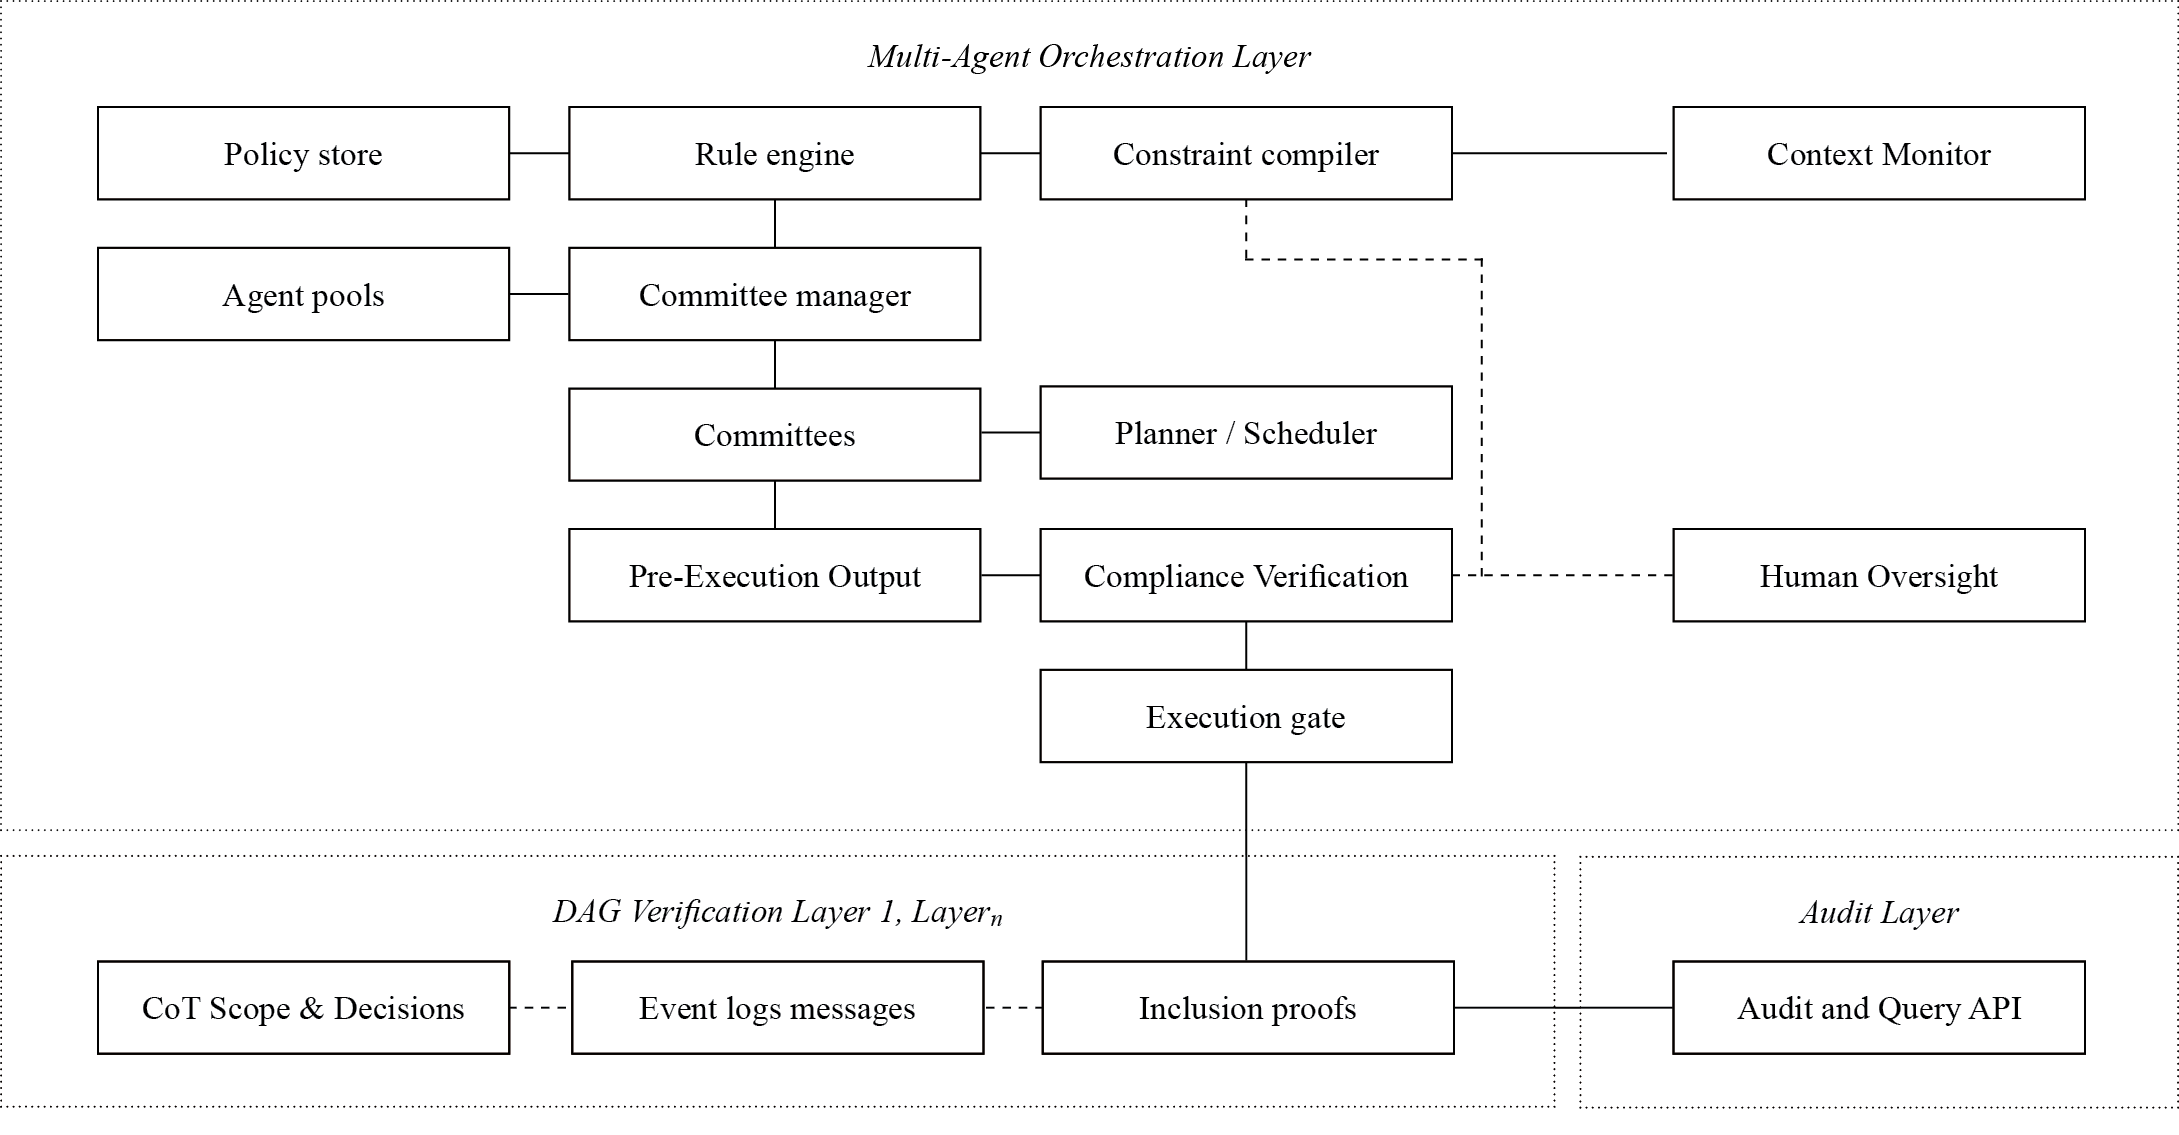
\includegraphics[width=\textwidth]{3-assets/1-User/AI_and_DLT_Enterprise_System.png}
    \caption{Layered orchestration architecture integrating the context-adaptive cooperation--competition parameter
    $\gamma_t$. The Policy and Governance components compute $\gamma_t$ via $f(\mathcal{S}_t, \mathcal{P}, \Theta)$
    and compile constraints $\{\mathcal{C}_x\}$. The Orchestration Layer plans and verifies outputs, while the DAG
    Verification Layer notarises Chain-of-Thought scopes, decisions, and constraint outcomes. The Audit Layer
    enables forensic and simulation queries.}
    \label{fig:orchestration-architecture}
\end{figure}
While existing multi-agent orchestration frameworks tend to address coordination, optimisation, or compliance as separate concerns, few combine them in a single architecture that treats the cooperation--competition balance as a governed, context-adaptive parameter. The design in Figure~\ref{fig:orchestration-architecture} embeds $\gamma_t$ directly into the decision loop, applies compliance checks before execution, and records all strategic changes with verifiable provenance. This integration closes two persistent gaps in the literature. The first is the absence of a mechanism for adjusting inter-agent posture along a continuum from fully cooperative to fully competitive in response to contextual triggers.  The second is the lack of a transparent link between those triggers, the orchestration decisions they influence, and
their eventual operational outcomes. Addressing both allows enterprise-scale multi-agent systems to remain strategically agile while demonstrably aligned with long-term viability objectives.

A Directed Acyclic Graph (DAG) is adopted as the notarisation substrate to avoid the latency bottlenecks inherent in block-generation intervals of conventional blockchains. For audit logs that are technical rather than financial, the confirmation delays and transaction fees typical of Layer~1 financial ledgers are poorly aligned with operational requirements. In the proposed model, events are minted into a Layer~2 DAG with negligible or zero transaction costs, allowing high-frequency, low-latency notarisation of decisions, constraint checks, and contextual triggers. Where minting costs are non-zero, a game-theoretic incentive design can be applied to favour comprehensive notarisation while retaining the ability to omit non-critical events. Let $\mathcal{E}$ be the set of events, $c(e)$ the minting cost of event $e \in \mathcal{E}$, and $v(e)$ its expected verification or audit value. The resulting notarisation preference function is given in Equation~\eqref{eq:dag-mint-preference}:
\begin{align}
\max_{\mathcal{E}' \subseteq \mathcal{E}} \quad & \sum_{e \in \mathcal{E}'} \big[ v(e) - \lambda \cdot c(e) \big]
\label{eq:dag-mint-preference}
\end{align}
Here, $\lambda$ captures the operator’s sensitivity to cost. By calibrating $\lambda$, the system can favour high-value, low-cost events while discouraging the omission of critical actions. Under realistic cost conditions, comprehensive notarisation can be made the dominant operational choice. The Layer~2 DAG can periodically anchor its state via Merkle tree commitments to a Layer~1 ledger, which may be either a general-purpose blockchain or a specialised ledger dedicated to AI system activity logs. In both cases, the economic model of the underlying ledger influences the completeness of notarisation. Within this framework, the DAG functions as a verifiable record of system activity and a primary source for forensic analysis, simulation replay, and regulatory audits.

In a dedicated DAG system, the vectorisation of smart contracts and stored hashes is proposed to enable AI agents to parse and reason over notarised content with greater efficiency and security. Representing contract logic and state proofs as vectorised structures allows faster retrieval and interpretation while ensuring compatibility with embedding-based reasoning systems. This can reduce parsing overhead and lower the risk of errors arising from ambiguous or inconsistent contract encoding. The feasibility of this approach, along with its performance trade-offs and security implications, must be validated through rigorous testing in realistic deployment environments. We regard this as a priority direction for future research, with the potential to strengthen the integration between notarisation layers and AI orchestration systems.

\subsection{Human Oversight as a Governance Primitive}\label{subsec:human-oversight}

Human oversight is embedded in the orchestration framework as a governance primitive, spanning the full operational lifecycle from policy definition to post-execution audit. In the proposed architecture, human actors interact with the system at points chosen for their alignment with governance objectives and risk profiles.

At the \emph{policy and strategy} level, human decision-makers establish baseline rules, operational constraints, and strategic priorities, including the cooperation--competition balance parameter $\gamma$. While $\gamma$ may be dynamically adjusted by the system in response to situational data $\mathcal{S}_t$, human operators retain the authority to refine or override these values when contextual insight exceeds the agents’ situational model. In volatile markets or emergent public health crises, for instance, a human may recalibrate the cooperative–competitive weighting on the basis of information not yet incorporated into the system state.

At the \emph{pre-execution} stage, humans participate in compliance validation for high-impact or high-risk actions. This may involve reviewing an \emph{output draft} from the orchestration layer, with compliance agents—human or AI—verifying adherence to regulatory, procedural, and ESG constraints before execution. Human reviewers act as an adaptive safeguard, addressing edge cases, interpretative ambiguities, or ethical considerations that fall outside the scope of formalised constraints.

At the \emph{audit and review} stage, human oversight complements AI-based auditing. Post-execution logs notarised in the DAG layer are accessible for forensic review, simulation replay, and regulatory reporting. High-volume routine verification may be handled algorithmically, whereas exceptional cases, disputed actions, or policy updates can trigger human-led audits. This dual-mode design combines the speed and coverage of automated verification with the interpretability and accountability of human review.

Integrating human oversight at multiple stages allows the system to incorporate human intuition, ethical reasoning, and domain expertise without diminishing the autonomy and scalability of the multi-agent fabric. Oversight frequency and depth can be adapted through scenario policies, increasing human involvement during periods of regulatory uncertainty or heightened reputational risk. By formalising oversight within the orchestration semantics rather than treating it as an ad hoc intervention, the architecture ensures that human judgement remains a governed, auditable, and strategically aligned element of system operation.

\section{Discussion and Theoretical Implications}\label{sec5}

The proposed architecture integrates a multi-agent orchestration framework with a context-adaptive cooperation--competition continuum, notarisation through a Layer~2 DAG, and governed human oversight. While these components have each been examined in prior work, their combination into a unified, policy-driven enterprise AI system represents a shift in both theoretical framing and operational design.

From a theoretical perspective, the cooperation--competition parameter $\gamma_t$ moves beyond static game-theoretic formulations toward a dynamic, context-aware representation. This formulation recognises that organisational strategy is not fixed along the competitive--cooperative axis, but evolves in response to market dynamics, environmental triggers, and internal strategic priorities. Embedding $\gamma_t$ as a tunable orchestration parameter brings the model closer to observed organisational behaviour in both profit-oriented and mission-oriented contexts. The continuum also creates a formal bridge between strategic management theory and multi-agent system design, supporting scenario modelling in which competitive advantage and cooperative stability are jointly optimised.

The use of a Layer~2 DAG as the notarisation substrate introduces additional theoretical considerations. It reframes distributed ledger technology in AI governance from a financial transaction ledger to a high-frequency, low-latency record of decision processes and constraint evaluations. This shift positions the ledger as a strategic memory that enables replay, forensic analysis, and policy refinement without the performance costs of Layer~1 blockchains. The game-theoretic cost–value function for notarisation in Equation~\eqref{eq:dag-mint-preference} formalises the trade-off between completeness and operational expenditure, allowing preferred behaviours to be embedded directly into the economic logic of the logging mechanism.

Embedding human oversight across multiple orchestration stages also carries theoretical significance. By defining human interaction points at policy formulation, pre-execution validation, and post-execution audit, the architecture treats oversight as a structural governance mechanism rather than a reactive safeguard. This ensures that human intervention is both traceable and integrated with operational constraints, supporting a hybrid governance model in which ethical reasoning and domain expertise complement algorithmic scale and consistency.

Taken together, the architecture operationalises concepts that have often been addressed separately in AI research: strategic adaptability, distributed trust infrastructure, and governed human–AI collaboration. The theoretical contribution lies in positioning these elements as interdependent components of an enterprise-grade, multi-agent AI system. This perspective offers new avenues for research on adaptive game-theoretic strategies, ledger-augmented governance mechanisms, and empirical studies of human oversight in complex socio-technical environments.

\section{Limitations and Future Research}\label{sec6}

The proposed architecture offers a coherent framework for enterprise-grade multi-agent AI orchestration, yet several limitations remain that merit further investigation.

The cooperation--competition continuum parameter $\gamma_t$ is theoretically well-founded but has not been empirically validated across heterogeneous organisational settings. Robust calibration of $\gamma_t$ will require longitudinal studies and controlled simulation experiments to test its stability, responsiveness, and resilience to strategic manipulation. The behavioural effects of abrupt $\gamma_t$ adjustments in high-stakes domains such as emergency healthcare or volatile financial markets remain largely unexplored.

The Layer~2 DAG notarisation mechanism addresses latency and transaction cost constraints, but introduces its own operational trade-offs. The cost–value formulation in Equation~\eqref{eq:dag-mint-preference} presumes accurate estimation of $v(e)$ and a stable cost-sensitivity parameter $\lambda$. In practice, both are likely to vary with shifting priorities, governance changes, and external pressures. Future work should examine adaptive strategies for tuning $\lambda$, as well as the implications of partial notarisation on the completeness and reliability of forensic records. The proposal to vectorise smart contracts and hashed proofs for AI-native access also requires targeted benchmarking to assess retrieval speed, parsing accuracy, and security performance under realistic deployment loads.

Human oversight, although structurally embedded at multiple orchestration stages, has not yet been assessed in terms of cognitive demand and process latency. Without careful design, oversight points could become operational bottlenecks when the complexity or frequency of agent actions exceeds feasible review capacity. A promising direction is the development of hybrid audit workflows that combine AI-assisted triage with selective human review, preserving both scalability and accountability.

Interoperability with existing enterprise systems and regulatory environments is another open challenge. Cross-layer anchoring strategies, jurisdiction-specific compliance rules, and sector-calibrated ESG thresholds will likely require domain-specific tailoring. These factors are critical for adoption in regulated industries and for ensuring cross-border operational validity.

\bigskip

\bigskip

\printbibliography

\swDeclarationsPage

\end{document}
